\documentclass[12pt]{article}
%Gummi|065|=)
\usepackage{amsmath, amsfonts, amssymb}
\usepackage[margin=0.5in]{geometry}
\usepackage{xcolor}
%\usepackage{graphicx}
%\usepackage{graphicx}
\newcommand{\off}[1]{}
\DeclareMathSizes{20}{30}{21}{18}

\newcommand{\myhrule}{}

\newcommand{\dash}{
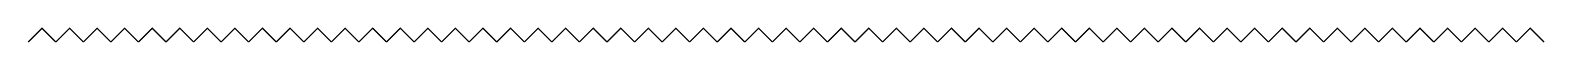
\begin{tikzpicture}[scale=0.35]
\foreach \x in {1,...,55}{
	\draw (\x,-0.25)--(\x+0.5,0.25)--(\x+1,-0.25);
}
\end{tikzpicture}
}

\usepackage{tikz}

\title{\textbf{ Examples:  Theta Functions}}
\author{John D Mangual}
\date{}
\begin{document}

\fontfamily{qag}\selectfont \fontsize{25}{30}\selectfont

\maketitle

\noindent  Conformal field theory is a central topic in mathematical physics\footnote{What does that even mean?  Here it means there are other math problems  in fields like Number Theory and Topology and Chern Simons Theory -- and specific sources -- which point to the paper we will review today. }.  What is Conformal Field Theory? \\
\dash
The rational gaussian model has a single scalar free field $\phi$ which is compactified on a circle with $R^2 \in \mathbb{Q}$.  \\ \\
This theory has a large group of symmetries -- an extension of the the $U(1)$ current algebra. \\ \\
The $N$ primary fields $[\phi_p]$ are vertex-operators with momentum $\frac{p}{\sqrt{N}}$ and $p \in \mathbb{Z}_N$. \\ \\
The fusion rules are $\phi_p \times \phi_q = \phi_{p+q}$ with $p,q \in \mathbb{Z}$.

\newpage

\noindent The discussion the last page is already quite problematic.  Why is $R^2 \in \mathbb{Q}$ , e.g. $R = \sqrt{3}$? \\ \\
It seems I have confused $\phi$ and $\varphi$.  These are related by the exponential function:
$$ \phi_p ( \textbf{c} )
= \exp \left( \frac{p}{\sqrt{N}} 
\int_\textbf{c} \partial \varphi \right)$$
this is such a nice looking integrals with nice properties:
$$ 
\phi_p ( \textbf{a} )
\phi_q ( \textbf{b} )
= 
e^{ 2\pi i \, pq/N}
\phi_q ( \textbf{b} )
\phi_p ( \textbf{a} )
$$
Now I want to know why these feel like the basic commutation operators from Quantum Mechanics:
$$ [x, p] = -i \hbar $$
and you can even prove these yourself, right? Let $p = -i\hbar \frac{d}{dx}$ then:
$$ \left[ x, i\hbar \frac{d}{dx} \right]f(x)
= i\hbar \left( x \frac{df}{dx}  - 
x\frac{df}{dx} + \frac{dx}{dx}f\right) = -i\hbar $$
Expect we are getting the exponentiated form.  That's it\footnote{I am not going to review anything more from Verlinde's paper -- I will be too busy making sense of these objects to discuss anything else.}

\newpage

\noindent Excuse me, Verline talks about the $S$ and $T$ operators.  The first one is clear:
$$ S: \chi_p \to \frac{1}{\sqrt{N}} \sum_{q \in \mathbb{Z}_N} e^{2\pi i \, pq / N}\chi_q $$
The only $\textit{S}$ and $\textit{T}$ operators that I know very well act on a Torus:
$$ S: 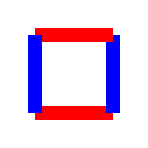
\begin{tikzpicture}
\draw[color= red, line width=5pt] (0,0)--(1,0);
\draw[color=blue, line width=5pt] (1,0)--(1,1);
\draw[color= red, line width=5pt] (1,1)--(0,1);
\draw[color=blue, line width=5pt] (0,1)--(0,0);
\end{tikzpicture} \to 
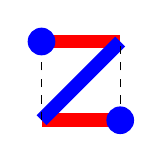
\begin{tikzpicture}
\draw[color= red, line width=5pt] (0,0)--(1,0);
\draw[color=blue, line width=5pt] (0,1) circle (1pt);
\draw[color= red, line width=5pt] (1,1)--(0,1);
\draw[color=blue, line width=5pt] (1,1)--(0,0);

\draw[dashed] (0,0)--(0,1);
\draw[dashed] (1,0)--(1,1);

\fill[color=blue] (0,1) circle (5pt);
\fill[color=blue] (1,0) circle (5pt);
\end{tikzpicture}
 $$
The other operator flips the torus (a technical term):
$$ T: 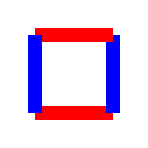
\begin{tikzpicture}
\draw[color= red, line width=5pt] (0,0)--(1,0);
\draw[color=blue, line width=5pt] (1,0)--(1,1);
\draw[color= red, line width=5pt] (1,1)--(0,1);
\draw[color=blue, line width=5pt] (0,1)--(0,0);
\end{tikzpicture} \to 
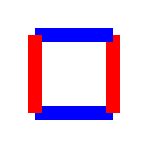
\begin{tikzpicture}
\draw[color=blue, line width=5pt] (0,0)--(1,0);
\draw[color= red, line width=5pt] (1,0)--(1,1);
\draw[color=blue, line width=5pt] (1,1)--(0,1);
\draw[color= red, line width=5pt] (0,1)--(0,0);
\end{tikzpicture}
 $$
This action lifts to \textbf{observable} that happens on that torus.  
$$ T: \chi_p \to e^{2\pi i \, p /N}\chi_p $$
With some effort these can happen on an octagon\footnote{Perhaps I should draw these by hand first!}\\
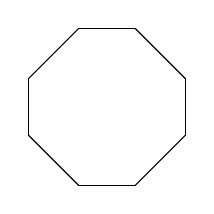
\begin{tikzpicture}
\draw (1, -0.356)--(1  , 0.356);
\draw (1,  0.356)--(0.356,   1);
\draw (0.356, 1) -- (-0.356, 1);
\draw (-0.356, 1)--(-1, 0.356);
\draw (-1, 0.356)--(-1,-0.356);
\draw (-1, -0.356)--(-0.356,-1);
\draw (-0.356, -1)--(0.356, -1);
\draw (0.356, -1)--(1, -0.356);
\end{tikzpicture}
...
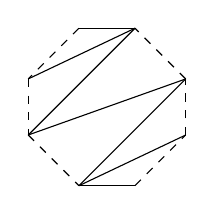
\begin{tikzpicture}
\draw[dashed] (1, -0.356)--(1  , 0.356);
\draw[dashed] (1,  0.356)--(0.356,   1);
\draw (0.356, 1) -- (-0.356, 1);
\draw[dashed] (-0.356, 1)--(-1, 0.356);
\draw (-1, 0.356)--(0.356,1);
\draw[dashed] (-1, 0.356)--(-1,-0.356);
\draw (-1, -0.356)--(1, 0.356);
\draw[dashed] (-1, -0.356)--(-0.356,-1);
\draw (-0.356, -1)--(0.356, -1);
\draw (-0.356, -1)--(1, -0.356);
\draw[dashed] (0.356, -1)--(1, -0.356);
\draw (-1, -0.356)--(0.356, 1);
\draw (-0.356,-1)--(1, 0.356);
\end{tikzpicture} \\
Verlinde's big result is: \textbf{the modular transformation $S$ diagonalizes the fusion rules}\footnote{See?  We can recite these formulas over and over many times with no idea what they mean :-)}
$$ \phi_p \times \phi_q = \phi_{p+q} $$

\newpage

\noindent How do we compactify the free scalar field on a circle?  \\ \\
Verlinde could have reminded us this scalar field was a section\footnote{or function} $\varphi: \mathbb{C}/(\mathbb{Z} + \tau \mathbb{Z}) \to \mathbb{R}$.  I think it's over $\mathbb{R}$.  It could be a complex valued field. \\ \\
Our torus is $S^1 \times S^1$ but I wish to remember the complex structure, so we remember\footnote{This space makes more sense after you've done a lot of cut-and-paste as on the previous page.} the number: $\tau \in \mathbb{C} / \text{SL}(2, \mathbb{Z})$  that section is generated by two transformations:
$$z \mapsto z + 1 \hspace{1in} z \mapsto - \frac{1}{z} $$
For that matter we could pick other very simple transformations and it makes a huge world of different.  For the record:
$$z \mapsto z + 1 \hspace{1in} z \mapsto - \frac{1}{4z} $$
That is because holomorphic function's don't just take partial derivatives.

\newpage

\noindent 

\begin{tikzpicture}
\node (A) at (0,0) {$f(z)$};
\node (B) at (7,0) {$f(z+dx)$};
\node (C) at (7,5) {$f(z+dz)$};
\node (D) at (0,5) {$f(z+dy)$};


\node at (8.5, 2.5) {\large $+ dy\, f'(z)$};
\node at (3, 0.5) {\large $+ dx\, f'(z)$};
\node at (3, 5.5) {\large $+ dx\, f'(z)$};
\node at (-1.5, 2.5) {\large $+ dy\, f'(z)$};

\draw[dashed] (A)--(B)--(C)--(D)--(A);
\end{tikzpicture}
It's hard to draw the picture of what holomorphic means... that the real and imaginary parts change in a compatible way.

\newpage

\noindent A \textbf{free field} or more specifically a \textbf{free boson} or \textbf{gaussian model} as an action:
$$ S = \int \mathcal{L} = \frac{1}{2\pi} \int \partial X \overline{\partial X} $$
and Ginsparg tells us the propagator should be:
$$ \langle X(z, \overline{z})\, X(w, \overline{w} )\rangle = - \frac{1}{2} \log |z - w| $$
What is a conformal field anyway?  Length behaves nicely under conformal mappings:
$$ ds^2 \mapsto \left( \frac{\partial f}{\partial z} \right)
\bigg( \frac{\partial \overline{f}}{\partial \overline{z}} \bigg) ds^2 $$
This field splits into a holomorphic and anti-holomorphic part\footnote{they are not complex conjugates... $x$ depends on $z$ and $\overline{x}$ depends holomorphically on $\overline{z}$.  Nature somehow requires the real and imaginary parts to behave separate but equal -- in reality creating two different worlds.}
$$ X(z, \overline{z}) = \frac{1}{2}( x(z) + \overline{x}(\overline{z}) ) $$
and I can't seem to find how $X$ behaves under conformal mappings $z \mapsto f(z)$.

\newpage

\noindent Conformal fields seem to be \textbf{representations of the Virasoro algebra} describing things that transform nicely under conformal maps:
$$ \ell_n: z \mapsto z + \epsilon \, z^n $$
I am looking for a formula for $x(z)$.  Reading many many times I try a formula I saw elsewhere:
$$ x(z) = \sum_{n = 0}^\infty a_n z^n $$
where $a_n$ is either an\footnote{The first version -- which makes the most sense to me -- I learned from Yuval Peres at PCMI 2007.  However it comes from work of Mikhail Sodin.}
\begin{itemize}
\item Gaussian random variable with mean 0 and norm $1$
\item a simple harmonic oscillator $[a_m, a_n] = \delta_{m, n}$
\end{itemize}
There is a way to pass between a Gaussian and harmonic oscillator that I reviwed before\footnote{There was a trick in symplectic geometry that takes one random walk and turns it into a harmonic oscillator. It could be the Distermaat-Heckman theorem.  When I wrote one thing it magically turned into the other.  This is a linear space, so it's reasonable to assume this will work in infinite dimensions.  } \\ \\
Oh, here is a free fermion:
$$ S = \frac{1}{8\pi} \int \psi \,\overline{\partial}\psi + \overline{\psi} \,\partial \overline{\psi} $$


\newpage

\noindent There is a lot to be unhappy with here.  And yet we continue.\\ \\
Section 8 of Ginsparg shows us how to put free bosons on a torus\footnote{ and the compactification means the image is a cylinder $S^1 \times \mathbb{R}$ and $X \equiv X + 2\pi r$.  All that seems to matter is the ring (order?) $\frac{1}{2r}\mathbb{Z} + \mathbb{Z}r $ and different $r$'s give the same range of numbers. I'm getting there}\dots  \\ 
\dash
My logic: all scalars are real numbers, so they all commute.  CFT has three similar-looking objects:
\begin{itemize}
\item fields
\item states
\item operators
\end{itemize}
A conformal field theory \textbf{is} a quantum field theory:
$$ \text{CFT} \subset \text{QFT} $$
A field could be a function $\phi: \mathbb{R}^2 \to V$ where $V$ is a vector space of some kind describing the feelings of the particle. \\ \\
The group of conformal transformations in the Eucliean plane should act on these fields in a nice way.  These nice actions are called \textbf{representations} -- and occasionally by other names. \\ \\
I am not the first person to lose sleep over a mathematical definition of CFT - there is also \textbf{Graeme Segal}, who has done much of that for me. \\
\begin{tikzpicture}[scale=0.35]
\draw (0,0)--(55,0);
\end{tikzpicture}
The representations of the conformal group are known as Verma modules.  \\ \\
Even easier (in flat space\dots) there is a recipe for quantizing the Hamiltonians\footnote{and now we complain that we don't really know or understand the Hamiltonian formalism.  My advice is to find an interesting motion that you like and then compute the Hamiltonian.  Advice \#2 -- they are always rotations. }  that one learns in the QFT class.   Start from Classical mechanics:
\begin{eqnarray*} \dot{q} &=& \; \;\,\frac{\partial H}{\partial p} = \{ q, H  \} \\ 
\dot{p} &=& -\frac{\partial H}{\partial q} = \{ p, H  \}  \end{eqnarray*}
 We simply decree that the Poisson bracket\footnote{Newton comes up with his awesome mechanics and we start solving free-body diagrams for two centuries.  Eventually we have trains and textiles and so forth.  If you solve these things all day, they kind of start to look the same.  Hamilton's equations (but first Lagrange) streamlined all of that.
 
As far as I can tell... the Hamiltonian is just a way to say ``total energy" -- and the Hamiltonian is \textit{generating} the flow of the position and momentum $(p,q)$.

From Hamiltonian's viewpoint, the position and conjugate momentum are interchangeable.  So we stop calling it $x(t)$ and call it $q(t)$ because it looks just like $p(t)$. } are replaced by Commutator brackets. 
\begin{eqnarray*} \dot{q} &=& [ q, H  ] \\  
\dot{p} &=&  [ p, H  ]  \end{eqnarray*}
and then our QFT class proceeds to write hundreds of pages of algebra without any insight.  \newpage

In QFT, the bosons still anti-commute.  If there is a boson we use a commutator:
$$ [a,b] = ab - ba $$
if we have a fermion we an anti-commutator:
$$ \{ a, b\} = ab + ba $$
which is just plain addition.

\newpage

\noindent For quantum field theory, the operator valued function\footnote{that's what Tong calls them}
$$ [\phi(x), \phi(y)] = 0 $$
and an eqation for the conjugate momentum 
$$ [\pi(x), \pi(y) ] = 0 $$
and the poisition and momentum should anti-commute
$$ [\phi(x), \pi(y) ] i \delta(x-y)$$
where $x, y \in \mathbb{R}^2$ and should behave nicely under the transformations of the conformal group.
$$ \phi: \mathbb{R}^2 \times V \to V $$
This still not write we basically took the Harmonic oscillator and added a new variable.  It is like we had a $2\times 2 $ matrix with variables $z \in \mathbb{C}$:
$$\left[ \begin{array}{rc} 
a(z) & b(z) \\ -\overline{b}(z) & \overline{a}(z) \end{array} \right]$$
\newpage

\noindent I don't think the book ever tells us exactly how $\phi$ acts on the space of states $|n(z) \rangle$ , or how the Virasoro algebra acts. \\ \\
and then I broke out Senechal.  I suppose all Verline has in mind are the eq on page 167:
$$ \phi(x + L, t) = \phi(x,t) + 2\pi m \, R $$
the free field goes around a cylinder $m$ times\footnote{If I wanted a ``free field" of some kind going around a circle --- as time progresses I just do a random walk... but on the condition that after a fixed amount of distance $L$ I have returned to where I started.  Since it is a circle I could have gone around any number of times.  That is the \textbf{winding number} $m \in \pi_1(S^1) = \mathbb{Z}$. }  and the Senechal-Di Francesco textbook furnishes us with a formula:
$$ \phi(x,t) = \phi_0 + \frac{n}{gRL} t + \frac{2\pi R m}{L} x + \frac{i}{\sqrt{4\pi g}} \sum_{k \neq 0} \frac{1}{k} \big( a_k e^{2\pi i k(x-t)/L} - \overline{a}_{-k} e^{2\pi i k (x+t)/L} \big) $$
the \textbf{homomorphic} part (using only $z$) is
$$ \partial x(z)
= x_0 - i \bigg( \frac{n}{4\pi g R} + \frac{1}{2} m R \bigg)\ln z + \frac{i}{\sqrt{4\pi g}}\sum_{k \neq 0} \frac{1}{k} a_k z^{-k}  $$
We will try again at some future time.  (Maybe soon!).

\fontfamily{qag}\selectfont \fontsize{12}{10}\selectfont


\begin{thebibliography}{}

\item Erik Verlinde. \textbf{Fusion rules and modular transformations in 2D conformal field theory.} \\ Nuclear Physics B
Volume 300, 1988, Pages 360-376

\item Luis Alvarez-Gaume \textbf{Topics in Conformal Field Theory} \\ \texttt{https://cds.cern.ch/record/204721/files/CERN-TH-5540-89.pdf}

\item Gregory Moore, Nathan Seiberg \textbf{Lectures on Rational Conformal Field Theory} \texttt{...}

\item Paul Ginsparg.  \textbf{Applied Conformal Field Theory} \texttt{arXiv:hep-th/9108028}

\item Mikhail Sodin. \textbf{Zeroes of Gaussian analytic functions} \texttt{arXiv:math/0410343}

\item Graeme Segal. \textbf{The definition of conformal field theory} See: \texttt{https://ncatlab.org/nlab/show/conformal+field+theory}


\end{thebibliography}



\end{document}